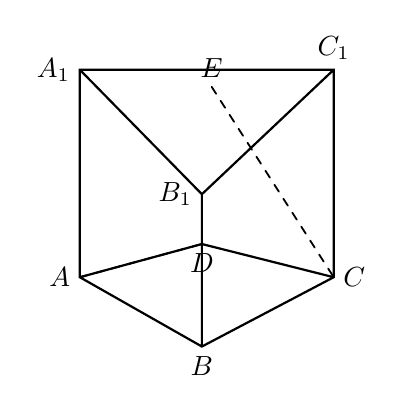
\begin{tikzpicture}[x=.62cm,y=.62cm,line cap=round,baseline=(current bounding box.center)]
  \coordinate (A) at (0,0); \coordinate (B) at (2.50,-1.42); \coordinate (C) at (5.20,0); \coordinate (B1) at (2.50,1.70); \coordinate (A1) at (0,4.25); \coordinate (C1) at (5.20,4.25); \coordinate (D) at (2.50,.68); \coordinate (E) at (2.70,3.90);
  \draw[line width=.8pt] (A)--(A1)--(C1)--(C)--(B)--cycle (A1)--(B1)--(C1) (A)--(D)--(C) (B1)--(D) (B)--(B1);
  \draw[dashed,line width=.65pt] (E)--(C) (A)--(D);
  \node[left] at (A) {$A$}; \node[below] at (B) {$B$}; \node[right] at (C) {$C$}; \node[left] at (A1) {$A_1$}; \node[above] at (C1) {$C_1$}; \node[left] at (B1) {$B_1$}; \node[below] at (D) {$D$}; \node[above] at (E) {$E$};
\end{tikzpicture}
